\section{Anhang}

\subsection{Bodediagramm eines Integrators}
\label{Bodediagramm eines Integrators}

Ein Integrator mit $G(s) = \frac{K}{s}$ hat seine Polstelle bei der Frequenz $\omega = 0$. Im Bodediagramm wird der Integrator so
dargestellt, dass bei Frequenz $\omega = 1$ die Verstärkung $20 \, \deci \bel \cdot \log_{10}(K)$ erreicht ist. 
Die Steigung beträgt $-20 \, \deci \bel / \mathrm{Dek}$ und die Phase ist konstant bei $\varphi = -\frac{\pi}{2}$

\begin{center}
    % Gain
    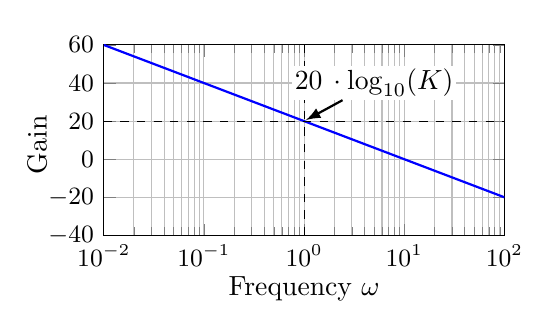
\begin{tikzpicture}
        [%
            scale = 1,
            >=latex
        ]
        \begin{axis}
            [%
                width=.55\columnwidth,
                height=4cm,
                % tick label style
                tick label style={font=\small},
                % x-axis
                xmode=log,
                xmin=0.01, xmax=100, ymin=-40, ymax=60,
                x label style={anchor=north, inner sep=0pt},
                xlabel=Frequency $\omega$,
                xmajorgrids=true,
                xminorgrids=true,
                % y-axis
                y label style={yshift=-1mm, anchor=south, inner sep=0pt},
                ylabel=Gain $\deci \bel$,
                ymajorgrids=true,
                yminorgrids=false
            ]

            % Plot
            \addplot[thick, color=blue, domain=0.01:100]{-20*log10(x)+20};
            
            % guide lines
            \addplot[dashed, color=black, domain=0.01:100]{20}; 
            \addplot [dashed, color=black] coordinates {(1, -40) (1, 60)};
           
            % Node / Label
            \node[inner sep=0pt] (p) at (1, 20) {};
            \node[fill=white, inner sep=1pt] (q) at (5, 40) {$20 \, \deci \bel \cdot \log_{10}(K)$};

            \draw[->, thick, color=black] (q) -- (p);
        \end{axis}
    \end{tikzpicture}
    % Phase
    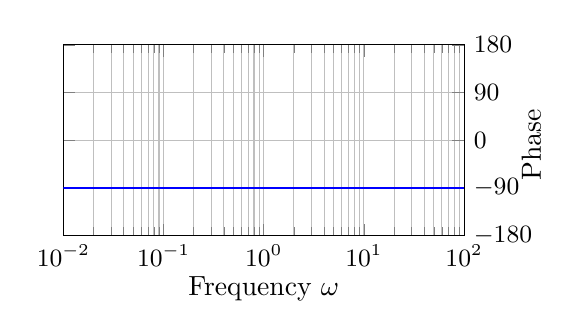
\begin{tikzpicture}
        [%
            scale = 1,
            >=latex
        ]
        \begin{axis}
            [%
                width=.55\columnwidth,
                height=4cm,
                % tick label style
                tick label style={font=\small},
                % x-axis
                xmode=log,
                xmin=0.01, xmax=100, ymin=-180, ymax=180,
                x label style={anchor=north, inner sep=0pt},
                xlabel=Frequency $\omega$,
                xmajorgrids=true,
                xminorgrids=true,
                % y-axis
                y label style={anchor=south, inner sep=0pt},
                ylabel=Phase $\degree$,
                yticklabel pos=right,
                ytick={-180, -90, 0, 90, 180},
                ymajorgrids=true,
                yminorgrids=false
            ]
            
            % Phase
            \addplot[thick, color=blue, domain=0.01:100]{-90};
        \end{axis}
    \end{tikzpicture}
\end{center}

 


\subsection{Bodediagramm eines Differenzierer}

Ein Differenzierer mit $G(s) = K \cdot s$ hat eine Nullstelle bei der Frequenz $\omega = 0$. Im Bodediagramm wird der Differenzierer so
dargestellt, dass bei Frequenz $\omega = 1$ die Verstärkung $20 \, \deci \bel \cdot \log_{10}(K)$ erreicht ist.
Die Steigung beträgt $20 \, \deci \bel / \mathrm{Dek}$ und die Phase ist konstant bei $\varphi = \frac{\pi}{2}$

\begin{center}
    % Gain
    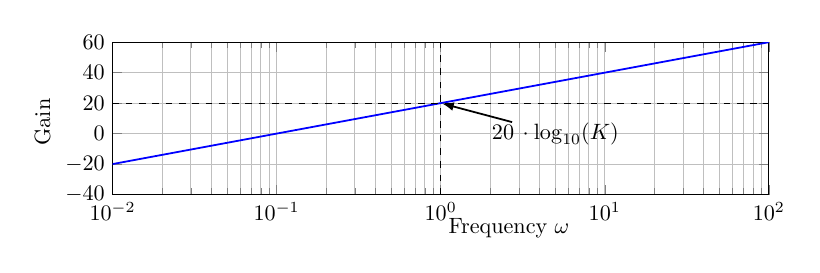
\begin{tikzpicture}
        [
            scale = 0.8,
            >=latex
        ]
        \begin{axis}
            [
                width=12cm,
                height=4cm,
                xmode=log,
                xmin=0.01, xmax=100, ymin=-40, ymax=60,
                x label style={anchor=west},
                xlabel=Frequency $\omega$,
                y label style={anchor=south},
                ylabel=Gain $\deci \bel$,
                xmajorgrids=true,
                xminorgrids=true,
                ymajorgrids=true
            ]

            % Plot
            \addplot[thick, color=blue, domain=0.01:100]{+20*log10(x)+20};
            
            % guide lines
            \addplot[dashed, color=black, domain=0.01:100]{20}; 
            \addplot [dashed, color=black] coordinates {(1, -40) (1, 60)};
           
            % Node / Label
            % \node (p) at (0.01, 20) {$20 \, \deci \bel \cdot \log_{10}(K)$};
            \node[inner sep=0pt] (p) at (1, 20) {};
            \node[inner sep=0pt] (q) at (5, 0) {$20 \, \deci \bel \cdot \log_{10}(K)$};

            \draw[->, thick, color=black] (q) -- (p);


        \end{axis}
        
    \end{tikzpicture}


    % Phase
    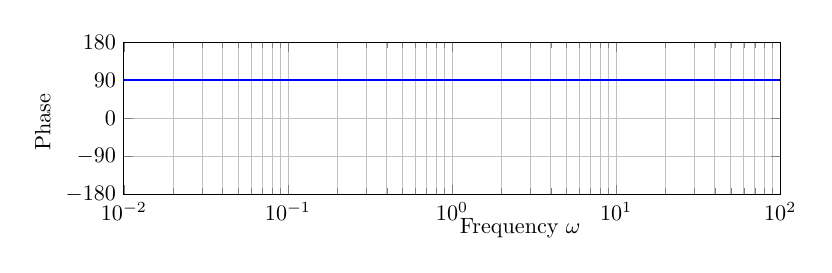
\begin{tikzpicture}
        [
            scale = 0.8,
            >=latex
        ]
        \begin{axis}
            [
                width=12cm,
                height=4cm,
                xmode=log,
                xmin=0.01, xmax=100, ymin=-180, ymax=180,
                x label style={anchor=west},
                xlabel=Frequency $\omega$,
                y label style={anchor=south},
                ylabel=Phase $\degree$,
                ytick={-180, -90, 0, 90, 180},
                % yticklabels={-180, -90, 0, 90, 180},
                xmajorgrids=true,
                xminorgrids=true,
                ymajorgrids=true
            ]
            
            % Phase
            \addplot[thick, color=blue, domain=0.01:100]{90};
                
        \end{axis}
            
    \end{tikzpicture}
\end{center} 


\subsection{z-Transformation}
\label{z-Transformation}

Die z-Transformation wird verwendet, um \textbf{diskrete} Signale in den Frequenzbereich zu transformieren.

\renewcommand{\arraystretch}{1}

\begin{center}
    \begin{tabular}{c c}
        \toprule
        \textbf{Zeitbereich}    & \textbf{Frequenzbereich}  \\
        \toprule
        \strut$u(k)$                  & $U(z)$                    \\
        \strut$u(k-1)$                & $z^{-1} \cdot U(z) = \frac{1}{z} \cdot U(z)$ \\
        \strut$u(k+1)$                & $z \cdot U(z)$\\
        \bottomrule
    \end{tabular}
\end{center}


\subsubsection{Z-Transformation mit Matlab}

\lstinputlisting{snippets/z_transformation.m}


\subsection{Fourier- bzw. Laplace-Transformation}

Die Fourier- und die Laplace-Transformation werden verwendet, um \textbf{kontinuierliche} Signale ein den Frequenzbereich zu transformieren.

\begin{center}
    \begin{tabular}{c c c}
        \toprule
        \textbf{Zeitbereich}            & \textbf{Frequenzbereich (Fourier)}                & \textbf{Frequenzbereich (Laplace)}    \\
        \toprule
        \strut$u(t)$                          & $U(\jimg \omega)$                                 & $U(s)$                                \\
        \strut$\int u(\tau) \, \diff \tau$    & $\frac{1}{\jimg \omega} \cdot U(\jimg \omega)$    & $\frac{1}{s} \cdot U(s)$              \\
        \strut$\frac{\diff}{\diff u(t)}$      & $\jimg \omega \cdot U(\jimg \omega)$              & $s \cdot U(s)$\\
        \bottomrule
    \end{tabular}
\end{center}
\renewcommand{\arraystretch}{1}

